
\documentclass[conference]{IEEEtran}

\usepackage{float} 
\usepackage{url}  
\usepackage{multirow}
\usepackage{subcaption}
\usepackage{booktabs}
\usepackage{cite}
\pagestyle{plain}
\usepackage{amsmath}
\usepackage{float}
\usepackage{tikz}
\usetikzlibrary{shapes.geometric, arrows, positioning}
\usepackage{placeins}


\ifCLASSINFOpdf
  \usepackage[pdftex]{graphicx}
\fi

\hyphenation{op-tical net-works semi-conduc-tor}

\begin{document}


\title{Lacuna Solar Survey Challenge: Counting Photovoltaic and Solar Panels from Aerial Imagery}

\author{\IEEEauthorblockN{\\ Hugo Veríssimo}
\IEEEauthorblockA{Complements of Machine Learning 24/25\\
University of Aveiro\\
Aveiro, Portugal\\
hugoverissimo@ua.pt}
\and
\IEEEauthorblockN{\\ João Cardoso}
\IEEEauthorblockA{Complements of Machine Learning 24/25\\
University of Aveiro\\
Aveiro, Portugal\\
joaopcardoso@ua.pt}}

\maketitle
\thispagestyle{plain}

\begin{abstract}
abstact
\end{abstract}

\begin{quote}
\small
\noindent
\textbf{Keywords:} EfficientNet, Object Detection
\end{quote}

\IEEEpeerreviewmaketitle


\section{Introduction}

Access to electricity and warm water is a basic necessity nowadays, and in developing countries the lack of a centralized distribution system makes access harder for everyone. Then it is essential for governments, non-governmental organizations and energy suppliers to understand how solar and photovoltaic panels are distributed throughout the territory to ensure proper planning and effective policy making. In this context, a challenge was created in the Zindi platform to develop a machine learning model capable of accurately detecting and counting the number of solar and photovoltaic panels in drone and satellite imagery.

In the present work, we have developed different approaches to the problem: taking a regression type approach, where images are analysed with EfficientNet type models and the target number of panels are provided; by identifying the panels through object detection and counting them afterwards; and by applying segmentation models to identify the regions of interest, analysing them and counting the panels.

EXPLICAR E FICAR BEM EXPLICITO: DUAS REGRESSOES: pan E boil

\section{state of the art?}

asdasdas

\section{Methodology}.

\subsection{Data description (com EDA)}

o dados, fornecidos pela propria competicao (citar), consistem em 4419 imagens, complementadas por metadata referente à origin da imagem e ao placement dos paineis, providing context on installation environments.

da totalidade destas imagens, 3312 (75\%) contêm indicacoes das delimitacoes de conjutnos de paineis e de boilers, atraves de poligonos, assim como a quantidade que se encontra dentro de cada qual. as restantes 1107 (25\%) nao têm esta informacao. Assim, por opcao da competicao, temos uma distribuicao de treino e teste de 75/25

\begin{figure}[H]
    \centering
    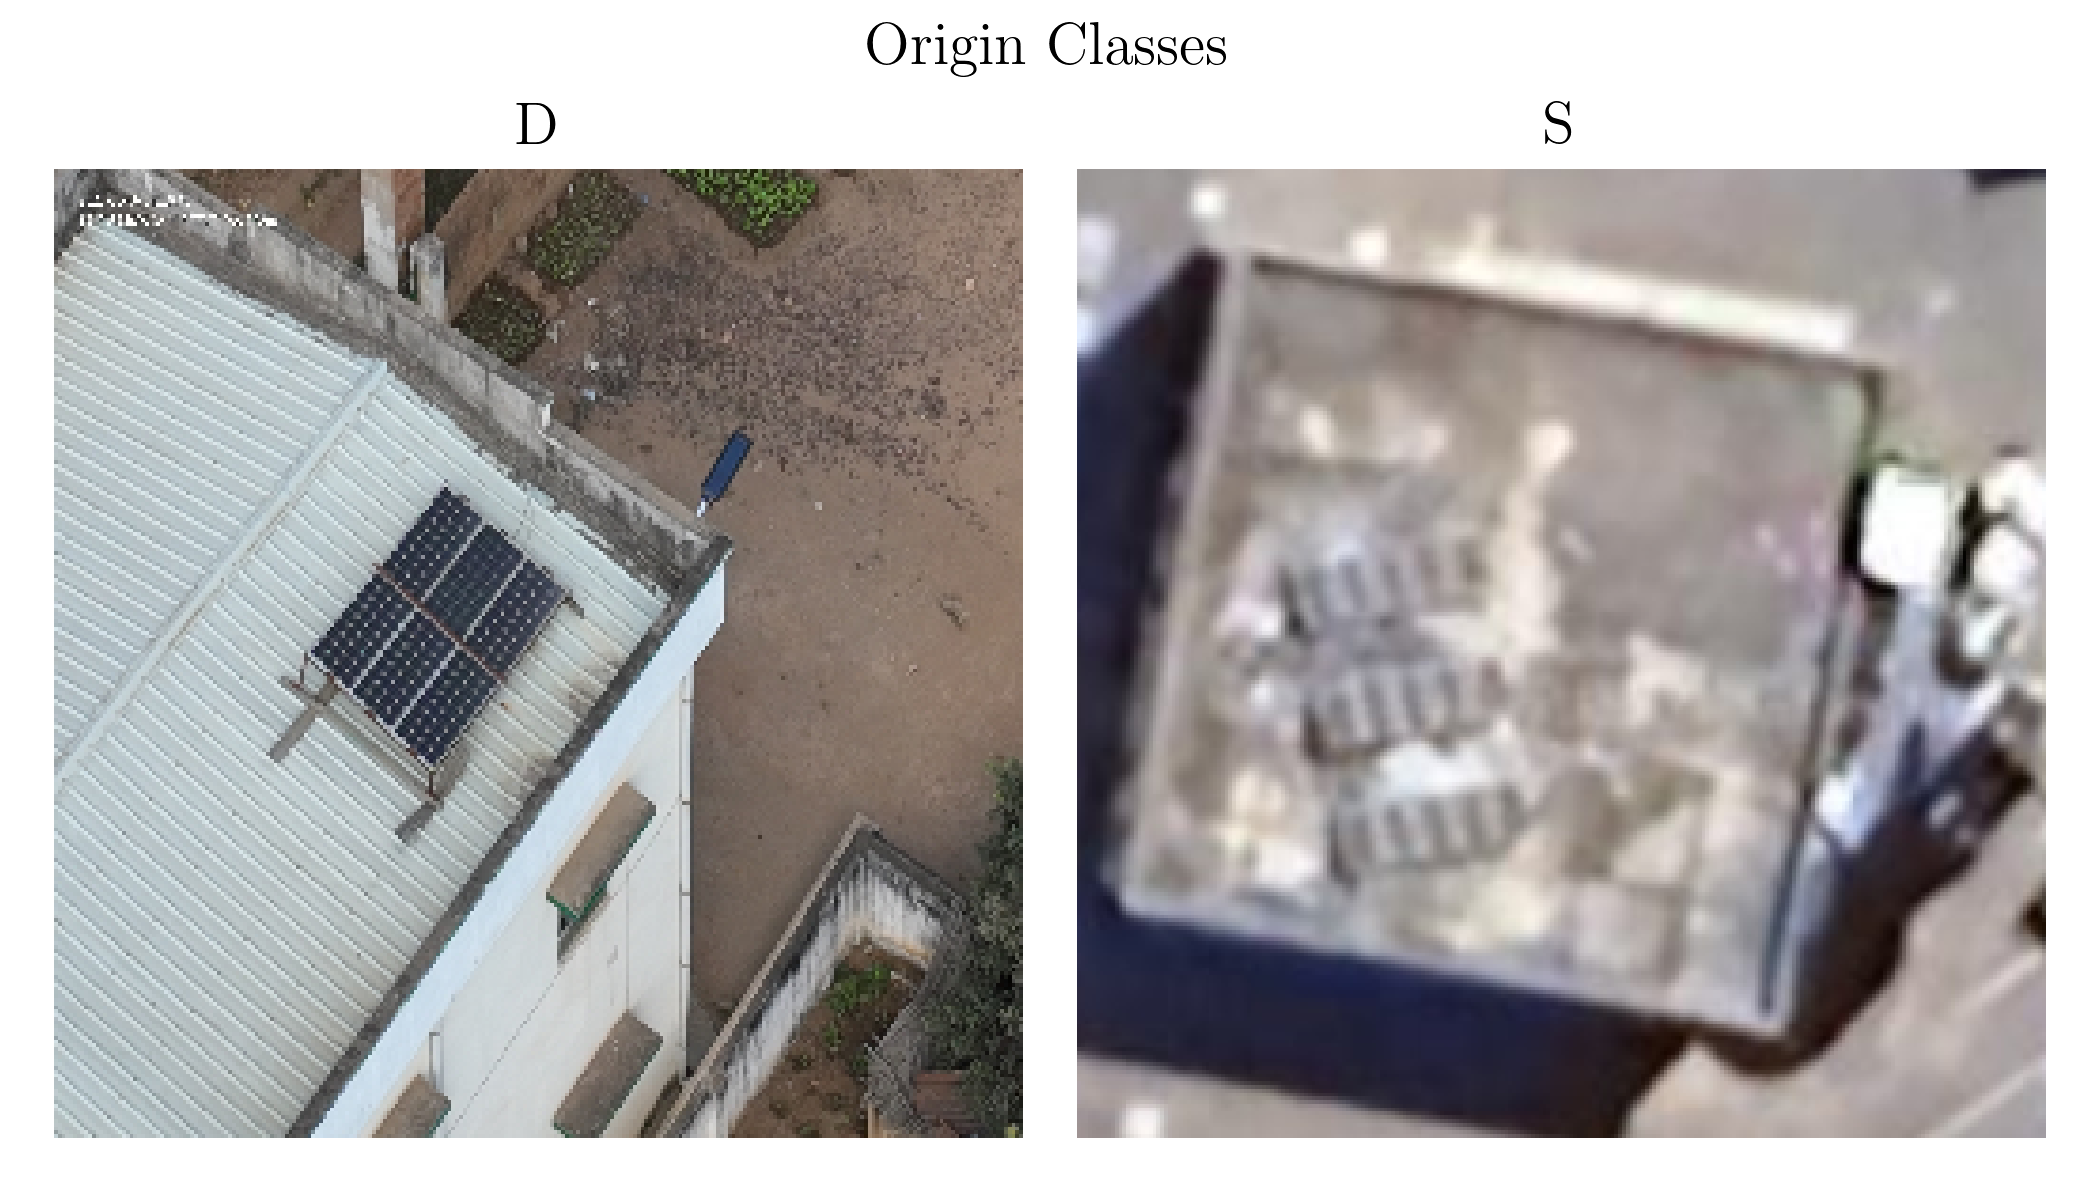
\includegraphics[width=1\linewidth]{assets/data_origin_classes.png}
    \caption{CAPTION CAPTION CAPTION CAPTION CAPTION}
    \label{fig:data_origin_classes}
\end{figure}

\begin{figure}[H]
    \centering
    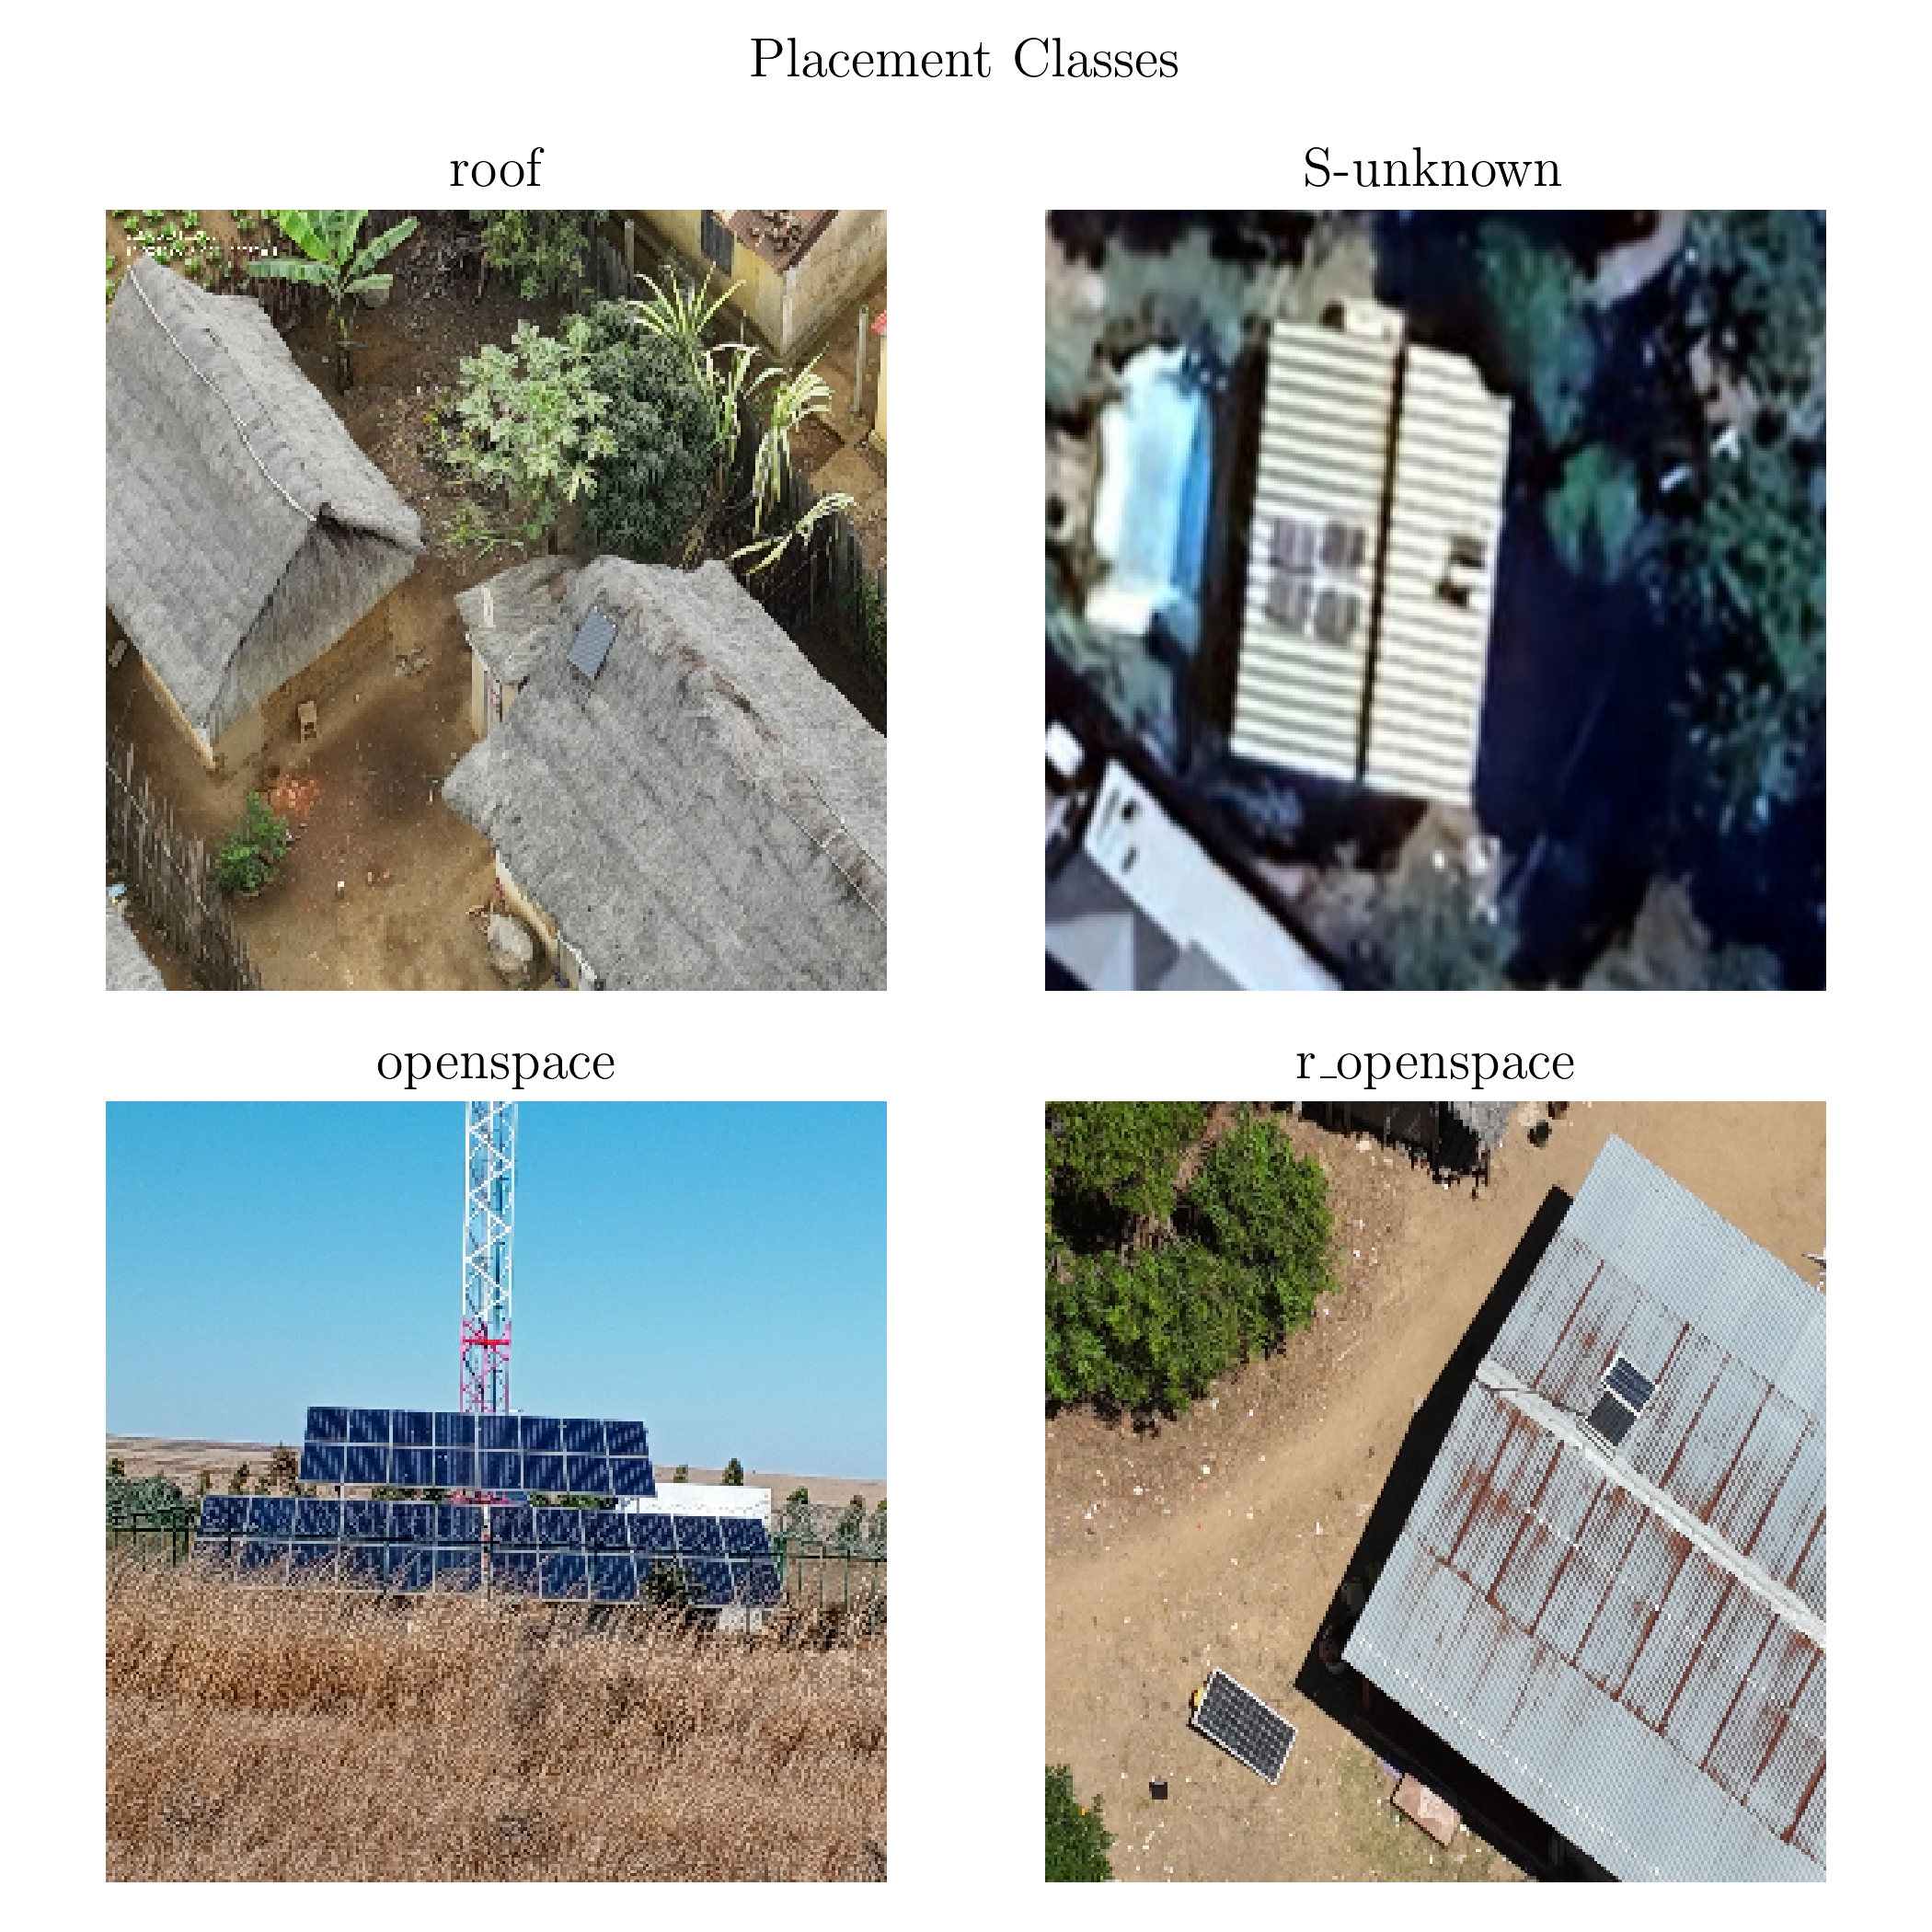
\includegraphics[width=1\linewidth]{assets/data_placement_classes.png}
    \caption{CAPTION CAPTION CAPTION CAPTION CAPTION}
    \label{fig:data_placement_classes}
\end{figure}

nas figuras \ref{fig:data_origin_classes} e \ref{fig:data_placement_classes} podem-se observar as classes de origin e de placement relativas as imagens. as origins da imagem podem ser drone image (D) or satellite image (S), while the placement classes (Installations) sao distribuidas por on rooftops or terraces (roof), satellite images where the specific placement could not be determined (S-unknown), in open courtyards or gardens (openspace), that span both rooftops and outdoor spaces (r\_openspace).


\begin{figure}[H]
    \centering
    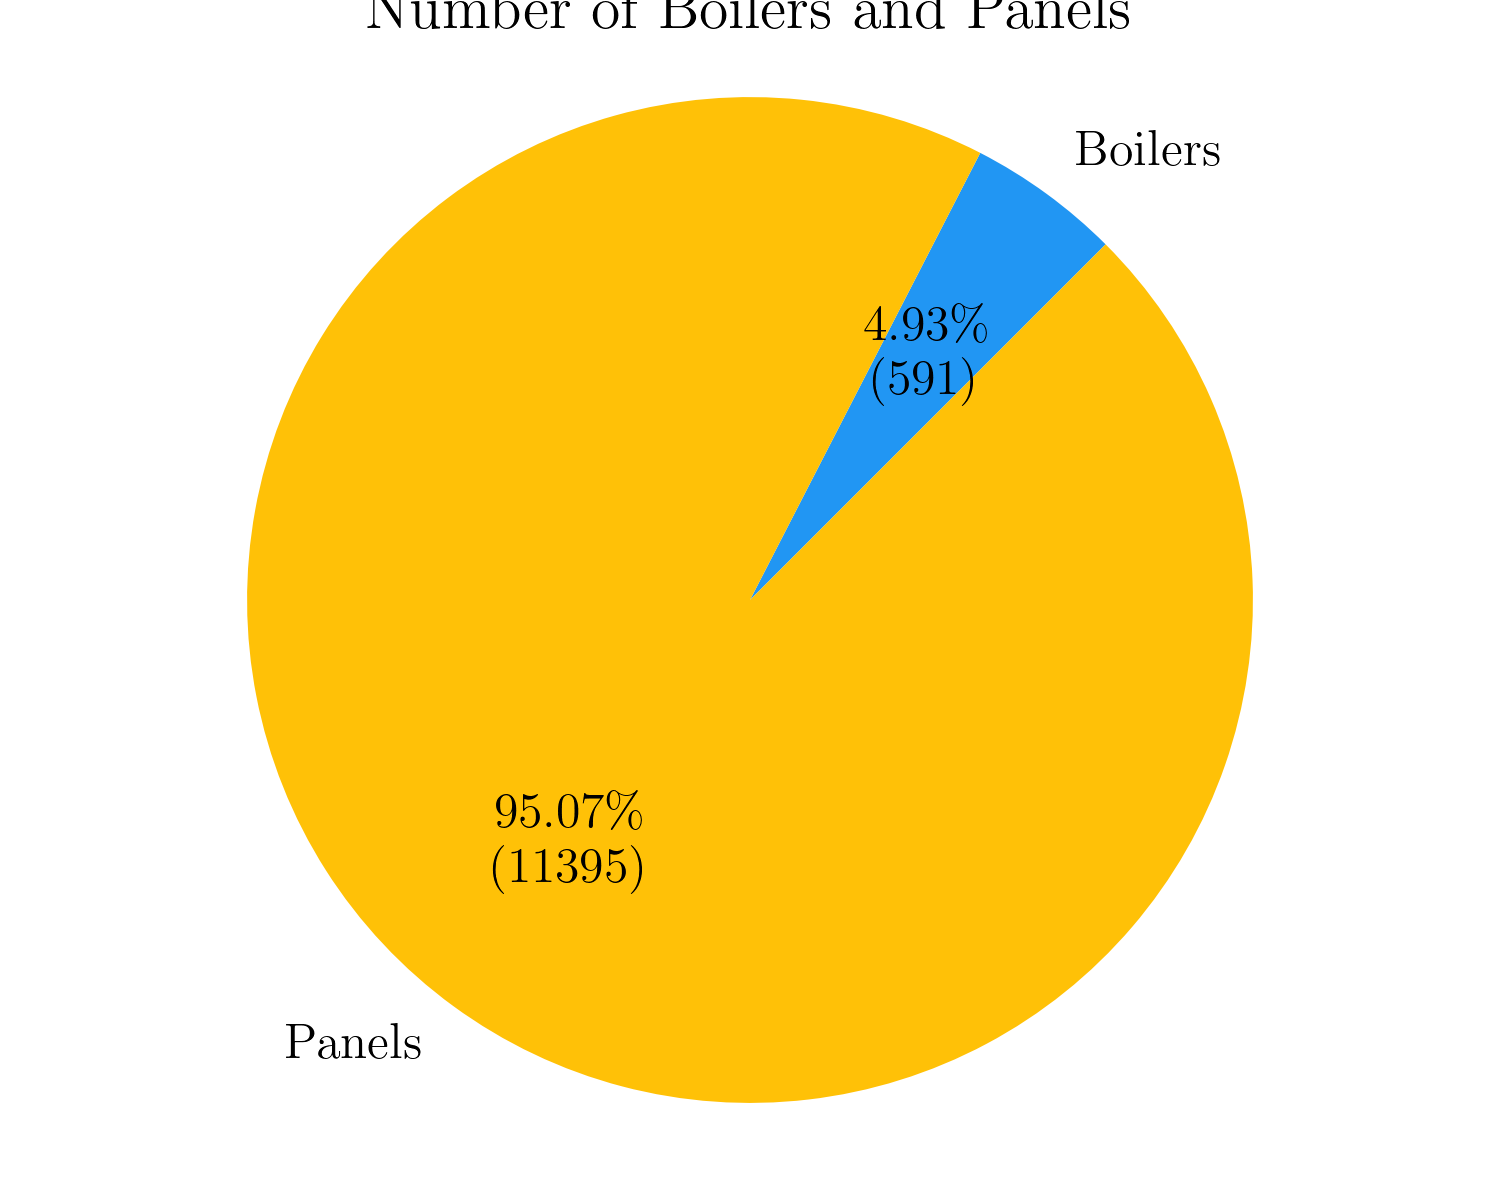
\includegraphics[width=1\linewidth]{assets/data_distribution.png}
    \caption{CAPTION CAPTION CAPTION CAPTION CAPTION}
    \label{fig:data_distribution}
\end{figure}

ademais, é também importante referir uma presença em maior peso de panels face ao numero de boilers, como se verifica na figura \ref{fig:data_distribution}

tendo em conta os poligonos referentes aos panels e boilers, também foi analisada a distribuicao da quantidade de paineis e de boilers naos poligonos que delimitam os conjuntos.

\begin{figure}[H]
    \centering
    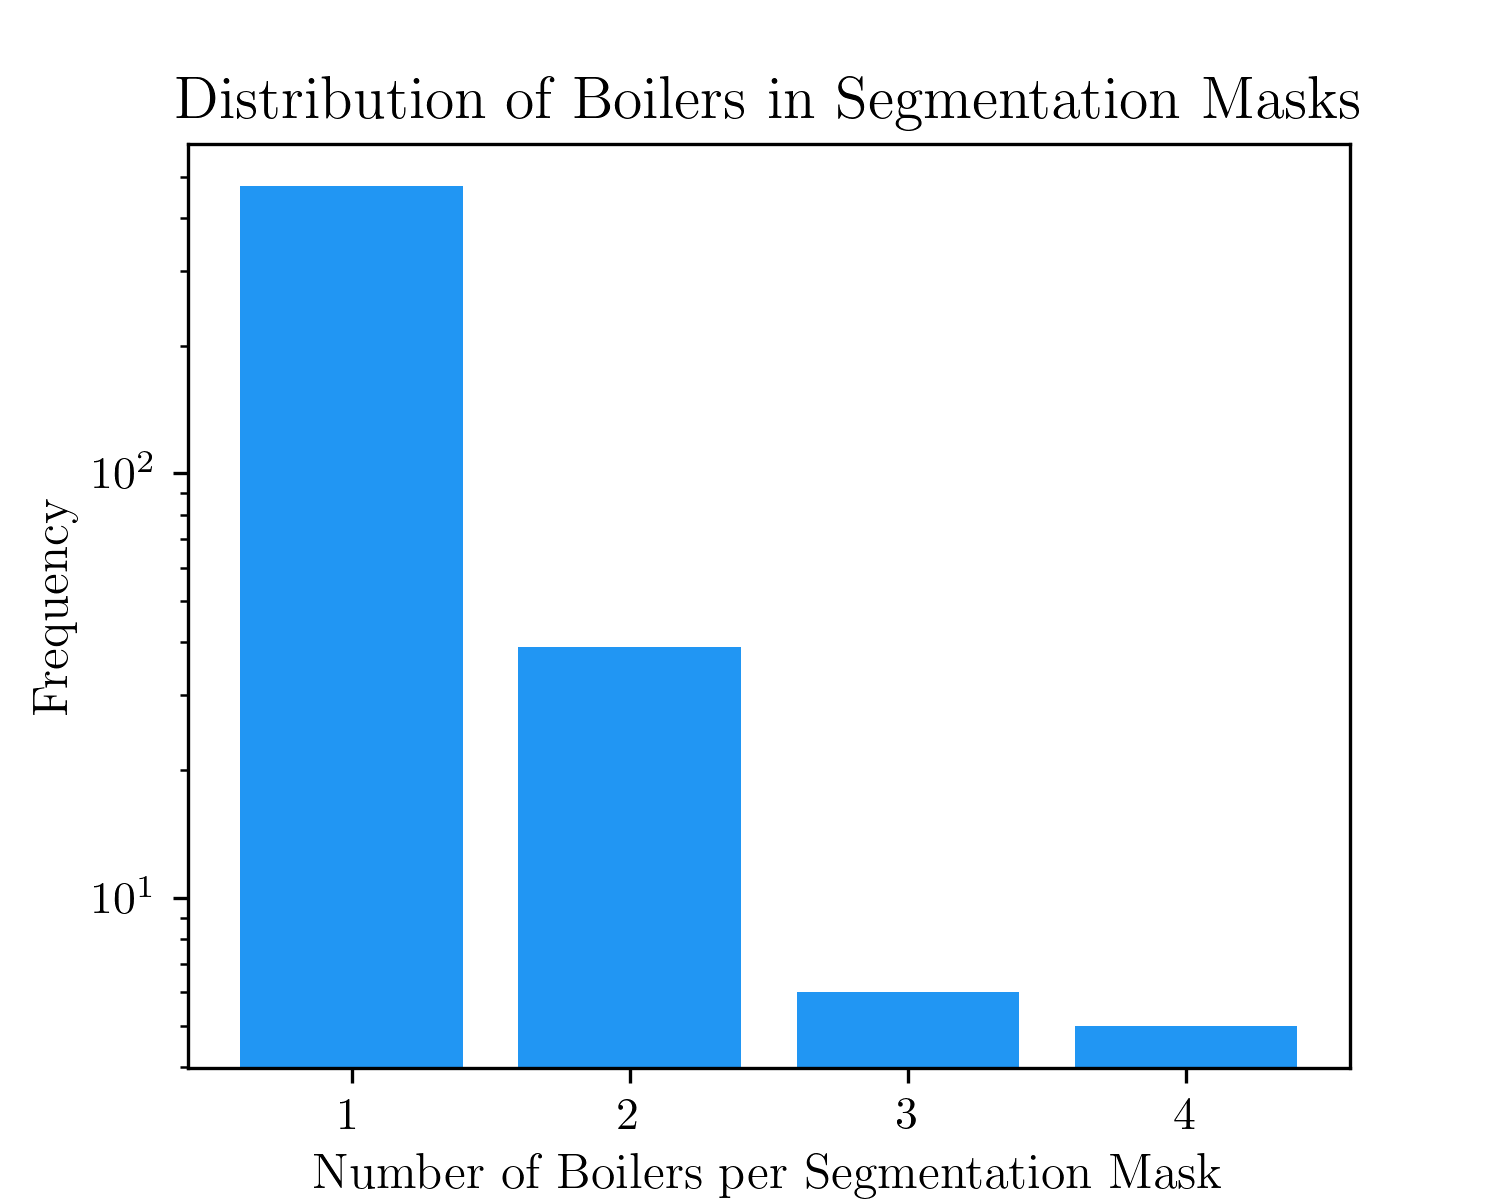
\includegraphics[width=1\linewidth]{assets/data_boil_distribution.png}
    \caption{CAPTION CAPTION CAPTION CAPTION CAPTION}
    \label{fig:data_boil_distribution}
\end{figure}

\begin{figure}[H]
    \centering
    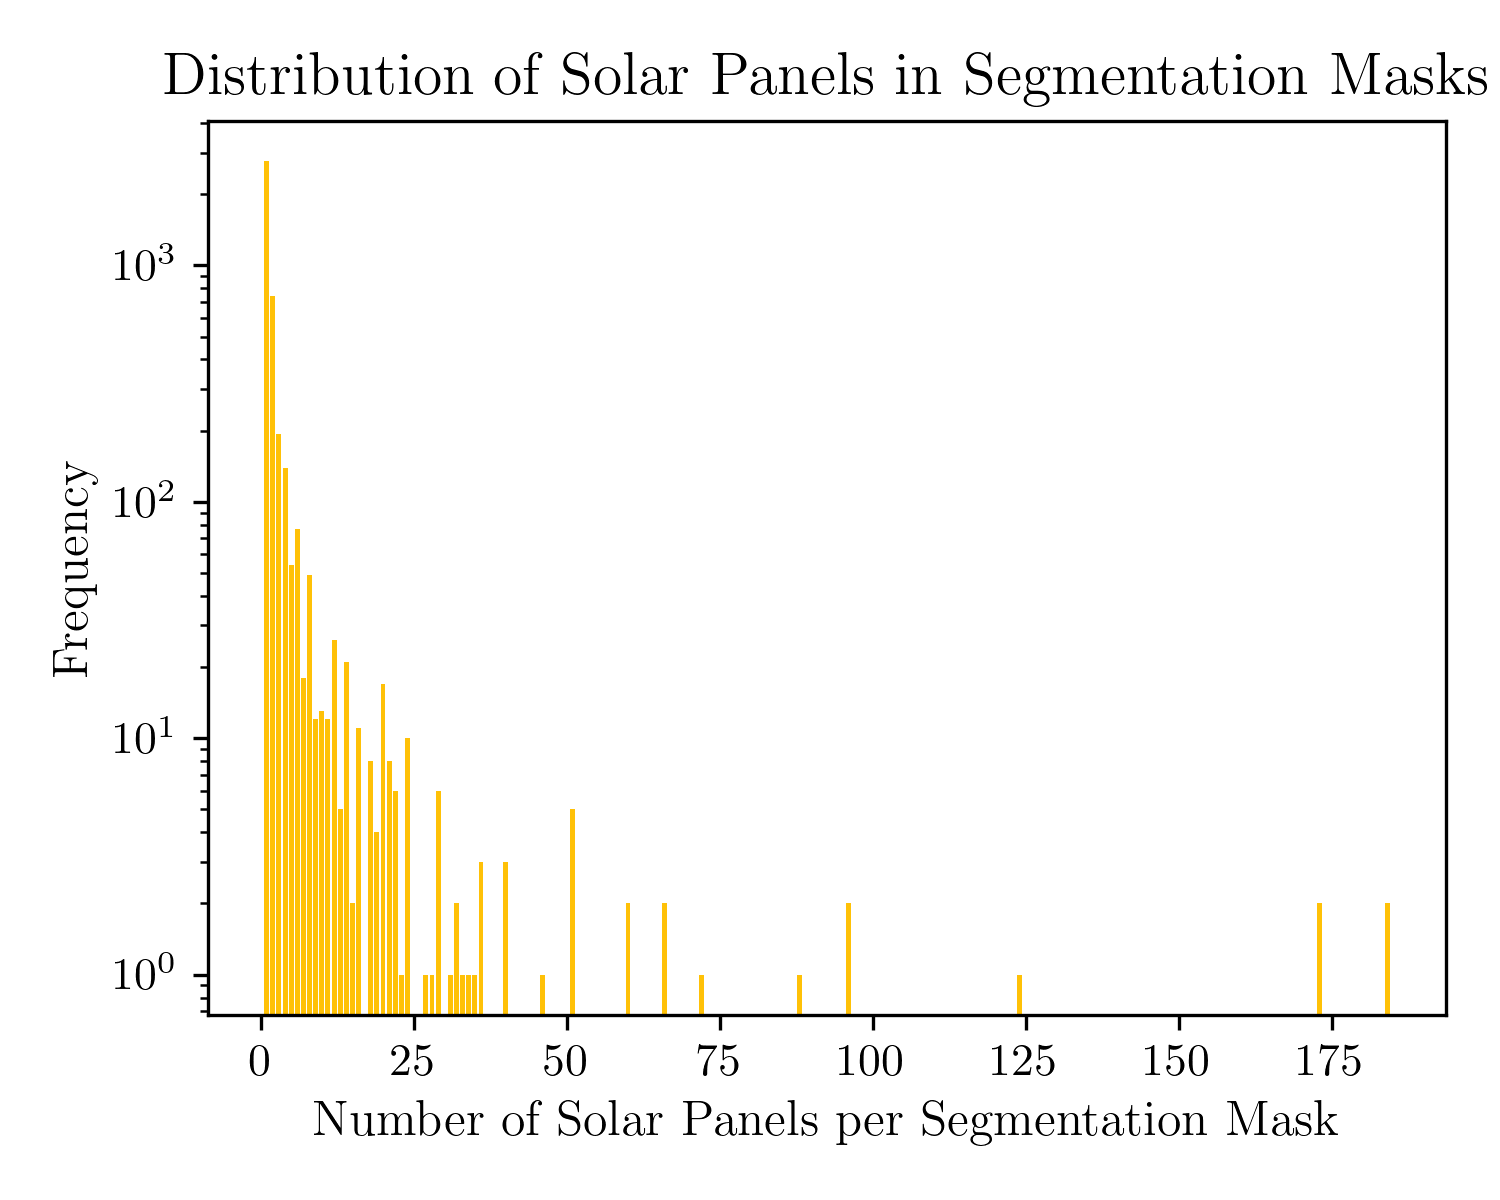
\includegraphics[width=1\linewidth]{assets/data_panel_distribution.png}
    \caption{CAPTION CAPTION CAPTION CAPTION CAPTION}
    \label{fig:data_panel_distribution}
\end{figure}

as figuras \ref{fig:data_boil_distribution} e \ref{fig:data_panel_distribution} revelam esta distribuicao, revelando que .... (fiquei sem inspiracao)


\begin{figure}[H]
    \centering
    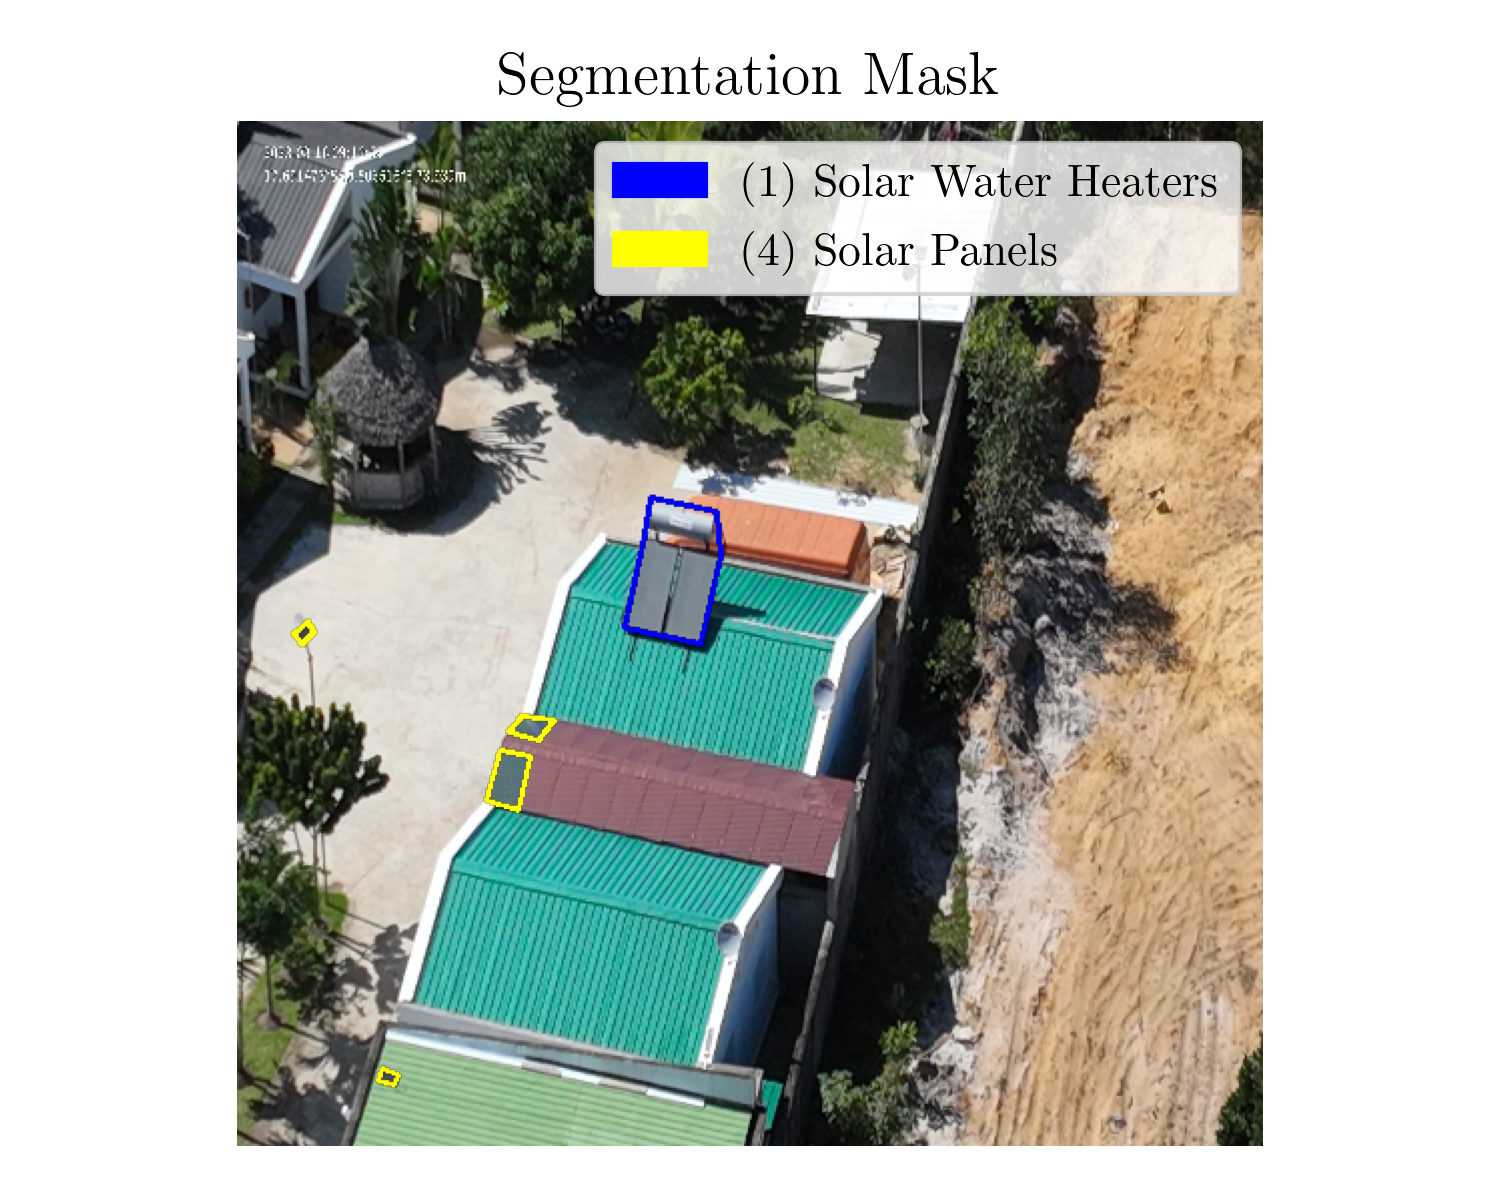
\includegraphics[width=1\linewidth]{assets/data_segmentation_mask.png}
    \caption{CAPTION CAPTION CAPTION CAPTION CAPTION}
    \label{fig:data_segmentation_mask}
\end{figure}

por fim, na imagem \ref{fig:data_segmentation_mask} pode-se verificar uma das imagens de treino e os respetivos poligonos referentes aos paineis e boilers convertidos numa mascara de segmentacao, onde se verifica a presença de 4 grupos de solar panels, sendo cada um destes um grupo unitário, e 1 grupo de boilers, tambem unitario.


\subsection{data: pre processamento e ques}

... n cheguei a escrever

- tratamento dos poliggos (str para lsita, tratar poligonos com letras no meio, juntar poligodos de imagens c o mesmo id, na mesma linha, pq antes era um poligono por linha)

- revisao manual de todas as imagens e correcao de poligonos mal desenhados ou localizados nas imagens
% https://zindi.africa/competitions/lacuna-solar-survey-challenge/discussions/25548
% GAJO QUE AJUDOU COM O ACETRTAR OS POLYGONS REFERENCIAR!

- cricao de classe python para correcao dos poligonos e facilitar leitura

- 263 imagens para o lixo

- separacao em 80/20 do dataset de treino em treino e validacao, visto q o teste é dado pelo concurso, online




data

\begin{figure}[H]
    \centering
    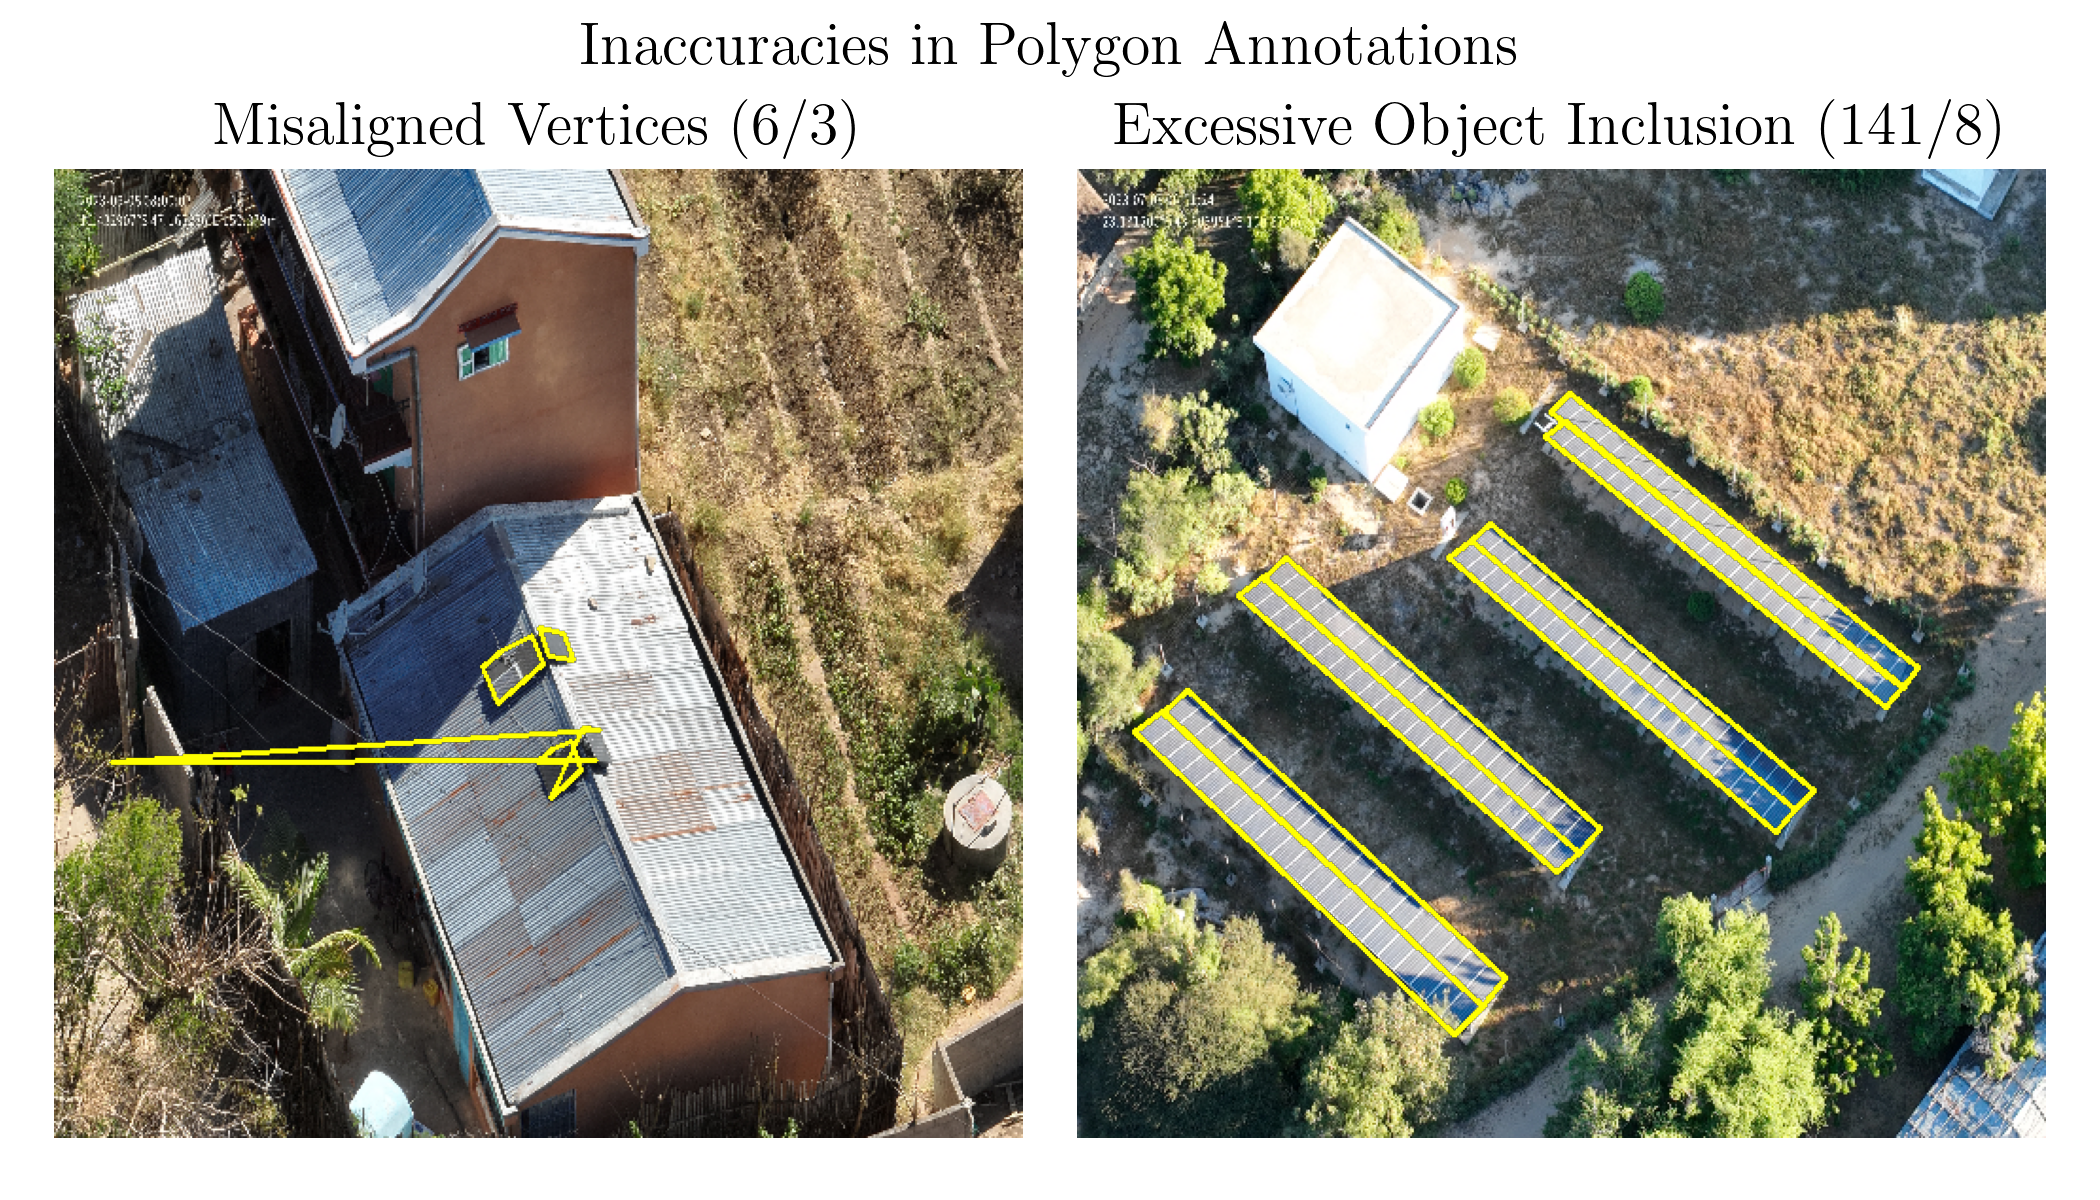
\includegraphics[width=1\linewidth]{assets/data_poly_problems.png}
    \caption{CAPTION CAPTION CAPTION CAPTION CAPTION}
    \label{fig:data_poly_problems}
\end{figure}

\begin{figure}[H]
    \centering
    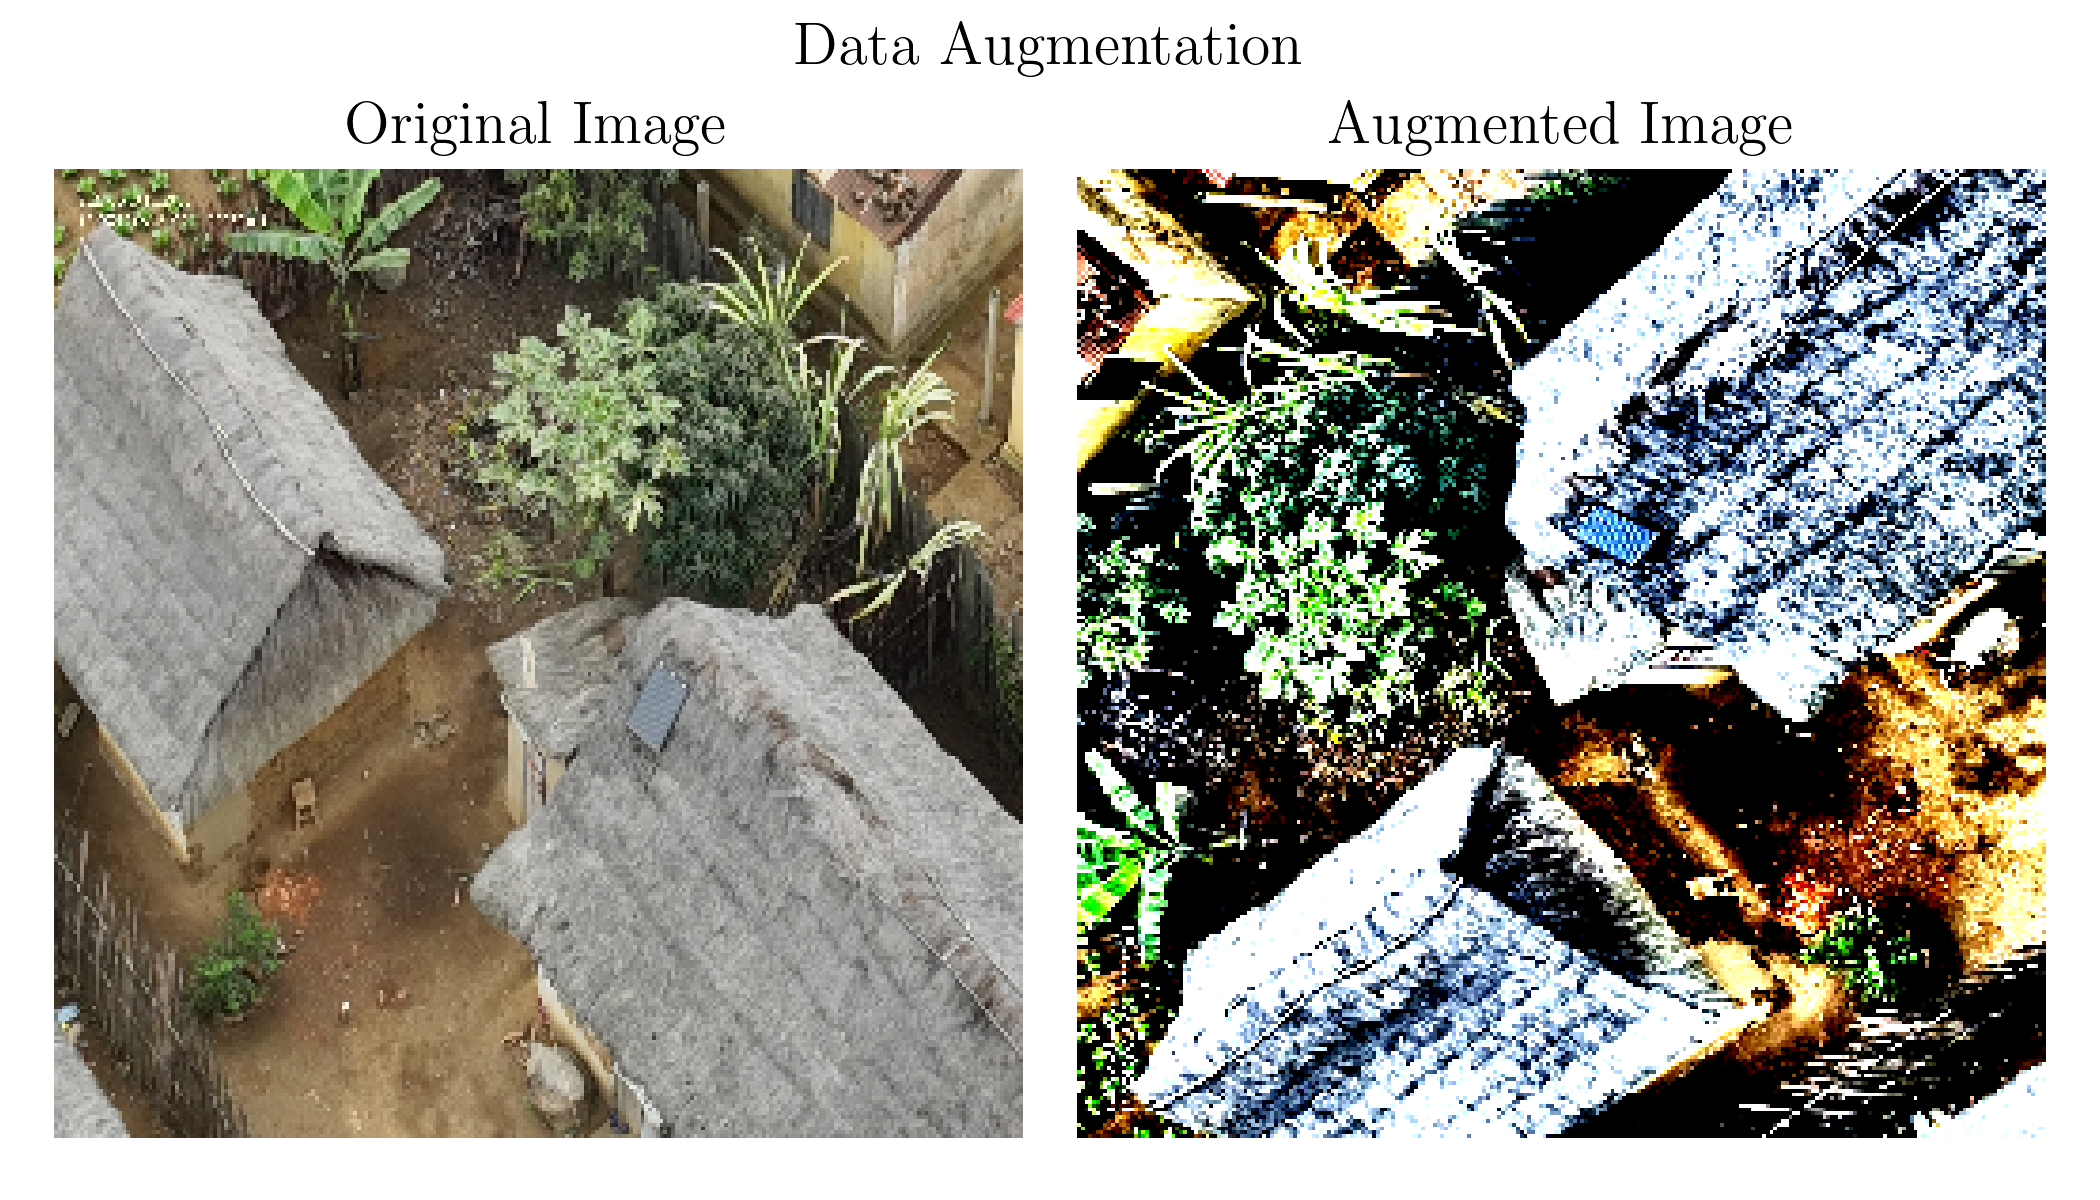
\includegraphics[width=1\linewidth]{assets/data_augmentation.png}
    \caption{CAPTION CAPTION CAPTION CAPTION CAPTION}
    \label{fig:data_augmentation}
\end{figure}


\subsection{Models implemented}

....




aaa


\section{djaisjd Models}

llalal

\subsection{03 model01 v04 - hugo}

- ler ficheiro train e test pickle

- fez se data augmentation e resize das imagens para 240x240

- input foi so a imagem e output foi so nr boil, nr pan

- modelo EfficientNetV2B0, imagenet, sem mudar os pesos originais

- adicionei global avg pool, dense, dropout e dps output

- usei random search para encontrar units do dense e learning rate, se calhar devia ter usado para o dropout tbm, too late

- usei early stopping, patiente 3, restore best wiehgts

-loss Huber delta 1, compiler adamW, métrica para melhor: mae

- dps de escolher o melhor, tem uns graficos no notebook das metricas

- o modelo n aprendeu bem as features q devia, underfitting

- \textbf{public score:} 3.040397919


\subsection{zulo40 models type}

% https://zindi.africa/competitions/lacuna-solar-survey-challenge/discussions/25675

\begin{figure}[H]
    \centering
    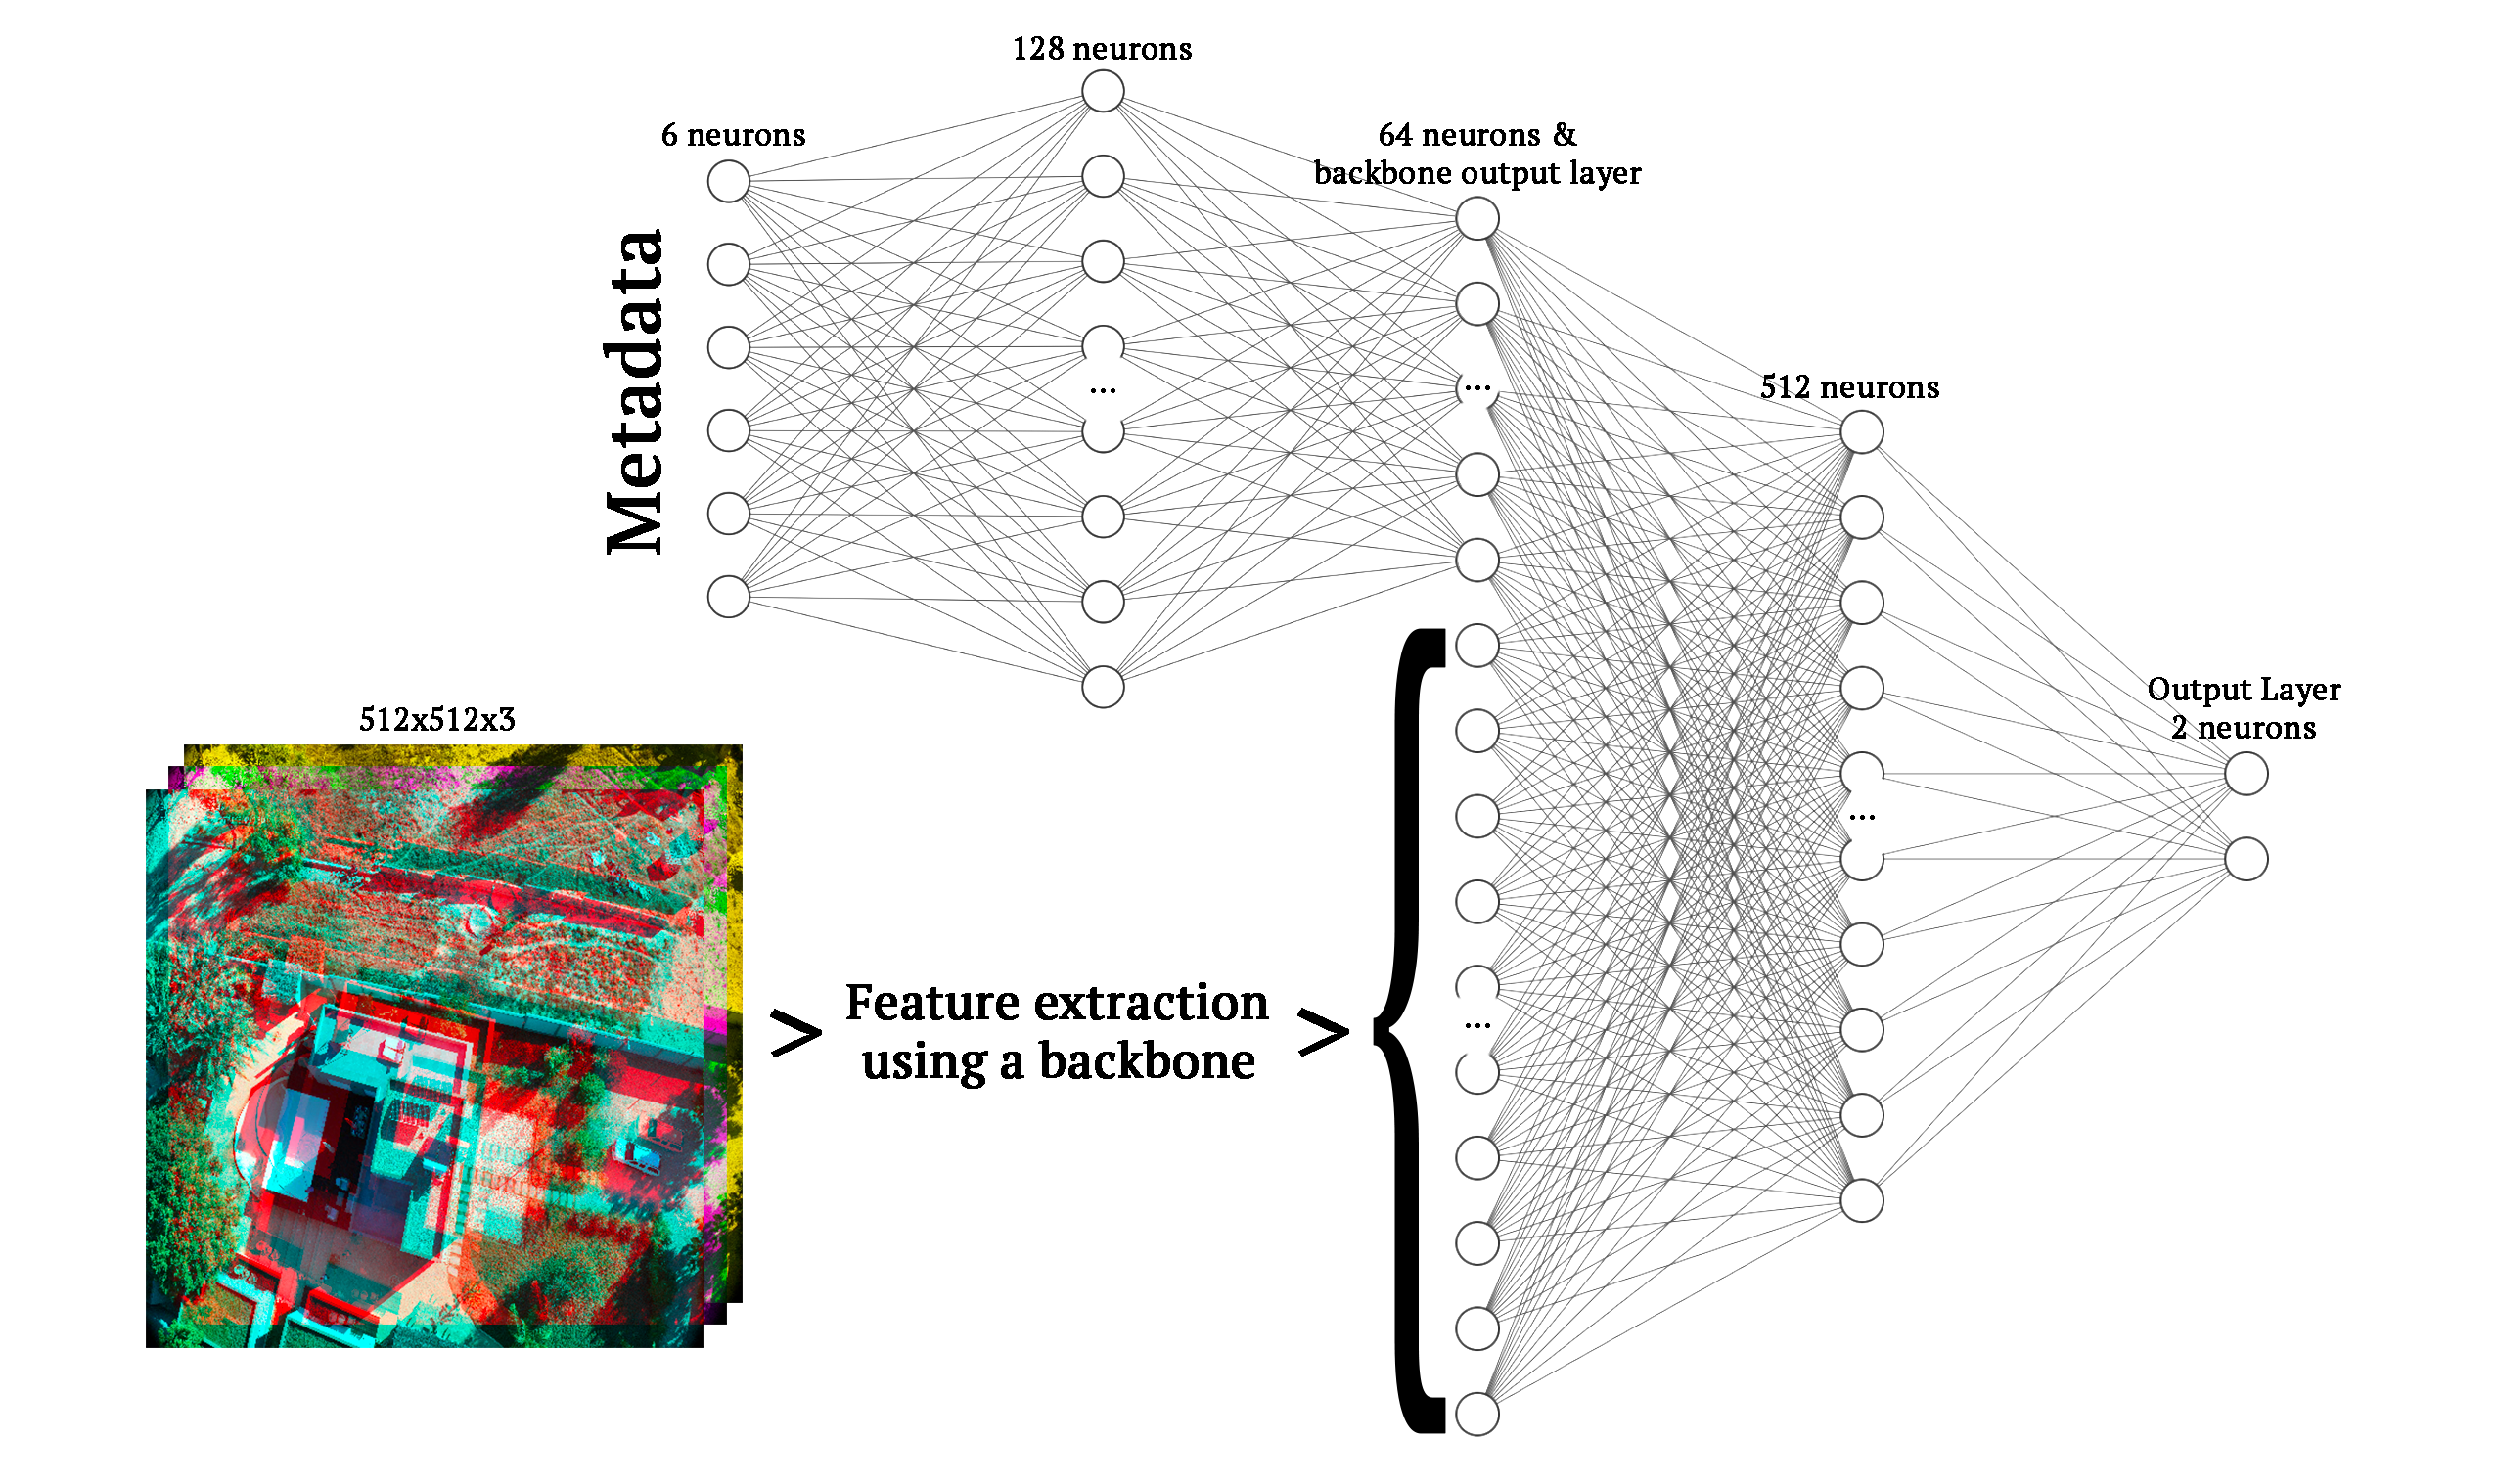
\includegraphics[width=1\linewidth]{assets/nn.png}
    \caption{CAPTION CAPTION CAPTION CAPTION CAPTION}
    \label{fig:nn}
\end{figure}

faz data augmentations

o cv q ele usa consiste em

- 3 folds

- para cada fold, um treino e um validacao (80/20), ajustanto um modelo em cada fold.

- no fim, junta os modelos (3, pq sao 3 folds) e faz a media das previsoes

- ou seja, usa 3 modelos como um só

ele usa Test-Time Augmentation (TTA), where the model makes multiple predictions on augmented versions of the same image (e.g., flipping, scaling, cropping). These predictions are later averaged to improve accuracy.

\subsection{yolo}

ideia inicial era fazer segmentacao de conjuntos de paineis e de boilers e posteriormente com outro modelo fazer contagem

problema foi q o modelo ao reconhecer paineis invidivudais, mesmo em conjuntos identificava individuais, levando ao mau desempenho do modelo

surgiu a ideia de criar 4 classeS: boiler, panel, conjunto de boileres, conjunto de panels, so q devido ao class imbalance o modelo teve resultados nao satisfatorios o suficente

METER GRAFICO IMABALANCE

entao decidiu-se rever o dataset e separar manualmente os poligonos em paineis e boileres indivudais, deixando de existir grupos de paineis

o yolo apresentou assim mt melhores resultados, apesar da reducao da dimensao do dataset em termos de imagens mas aumento de amostras do que realmente sao paineis e boilers individuais


fazer ja learning curve ou correr de novo last yolo?

IDEIA: correr de novo o last yolo, mas mudar hyperparemtros (lernaring rate, adamw, etc.), a ver se temos uma solucao melhor



\section{faa02 ig}



\begin{table}[H]
\centering
\caption{Error metrics for the train and test set (CF-LR), along with the number of samples for each.}
\label{tab:model01_results}
\begin{tabular}{lccc}
\toprule
\textbf{Dataset} & \textbf{RMSE} & \textbf{MAE} & \textbf{Support} \\
\midrule
Train Set & 0.58842 & 0.44604 & 80668 \\
Test Set & 1.24037 & 0.90651 & 20168 \\
\bottomrule
\end{tabular}
\end{table}

\section{Discussion} 

\subsection{Performance Metrics}

discussao


\section{Conclusion}

conc


\section*{Work Load}

Both authors contributed equally to the project.

\bibliographystyle{IEEEtran}
\bibliography{references}

\end{document}



